\section{Projektstyring}
\subsection{Rollefordeling}
\begin{table}[H]
  \centering
\begin{tabular}{l|l}
           & Roller:                                                \\ \hline
Alexander: & Visionsansvarlig, dokumentarist, strukturering         \\ \hline
Andreas:   & Konceptartist, informationssøgning                     \\ \hline
Jeppe:     & Produktansvarlig, programmør, artistsupervisor, vision
\end{tabular}
\caption{Viser rollefordelingen for vores projekt.}
\end{table}
\subsection{Tidsplan}
Vores tidsplan er håndteret via GitHubs indbygget funktion, se forneden, dog er den opdateret version her:
\begin{figure}[H]
  \centering
  \fbox{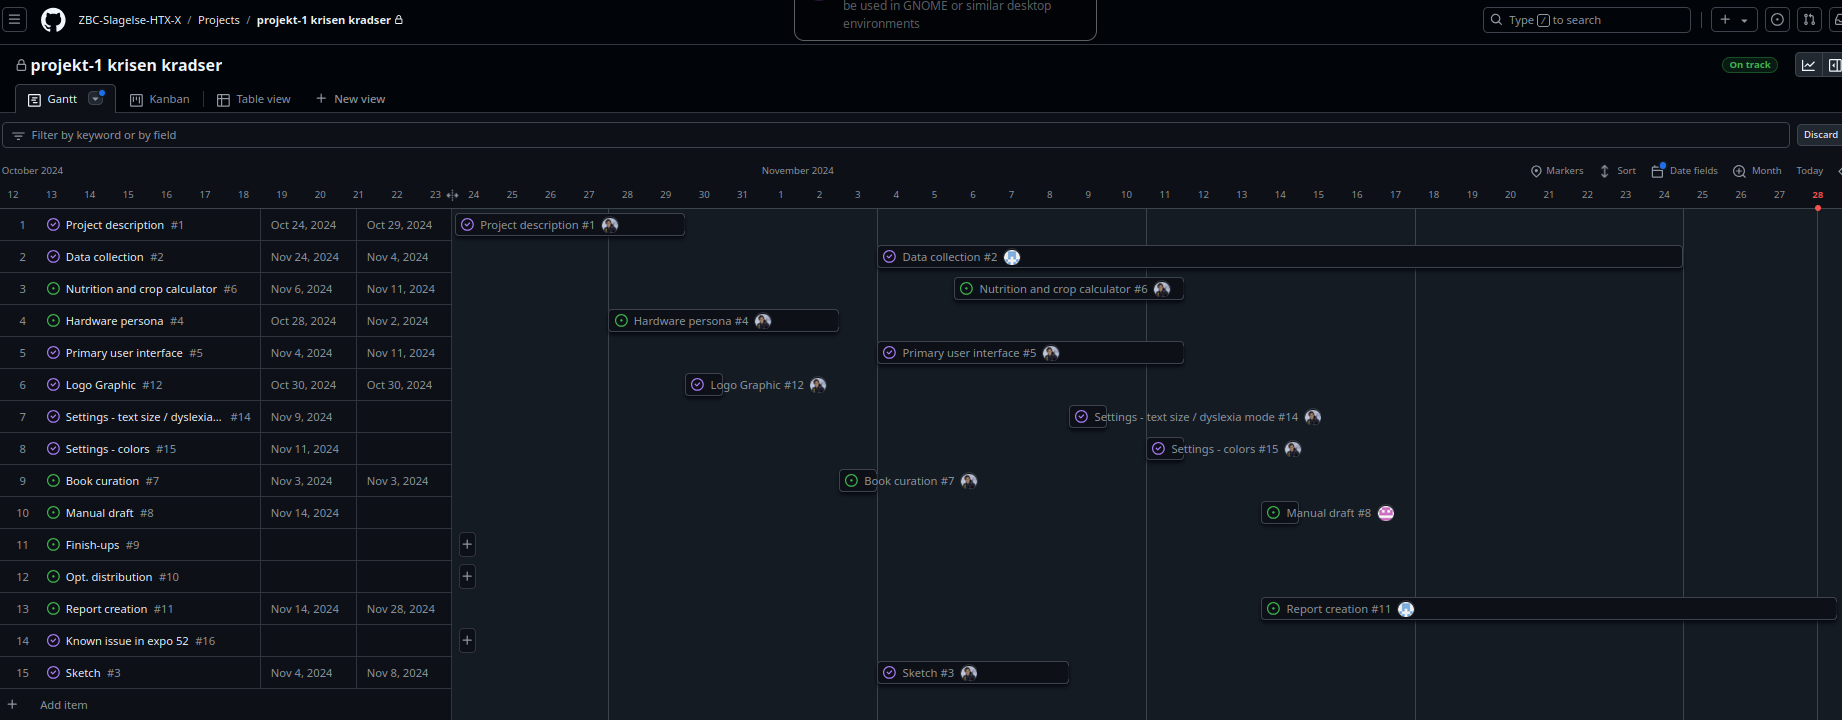
\includegraphics[width=\textwidth]{assets/section_2/2024-11-28_14-25.png}}
\end{figure}

Link til aktuel tidsstyring:
\subsection{Projektmappe}
Link: \href{https://github.com/ZBC-Slagelse-HTX-X/teknologiprojekt-1---Krisen-kradser/tree/main}{Vores GitHub fil}
